\documentclass[11pt,final,ENIB]{sdm}
\usepackage{graphicx}
\usepackage{subcaption}
\usepackage{textcomp}
\usepackage[francais,frenchb]{babel}

%numeroter les pages
\pagestyle{plain}

\title{Apprentissage profond et s\'eries temporelle}
\author{Arthur \textsc{Le Guennec}}
\supervisorOne{Romain \textsc{Tavenard}}
\supervisorTwo{Simon \textsc{Malinowski}}
\team{OBELIX}
%One of:
% ens-Rennes  esir    insa-rennes logoENIB  rennes1  UBO
% enssat header logo_ENIB   logoUbs   tel-br supelec

\school{logoENIB}



% the domain should be one or two of
% Technology for Human Learning 
% Artificial Intelligence				***** 
% Computer Arithmetic
% Hardware Architecture
% Automatic Control Engineering
% Bioinformatics 
% Biotechnology
% Computational Complexity 
% Computational Engineering, Finance, and Science
% Computational Geometry 
% Computation and Language 
% Cryptography and Security 
% Computer Vision and Pattern Recognition
% Computers and Society 
% Databases 							*****
% Distributed, Parallel, and Cluster Computing 
% Digital Libraries
% Discrete Mathematics 
% Data Structures and Algorithms 
% Embedded Systems 
% Emerging Technologies 
% Formal Languages and Automata Theory 
% General Literature 
% Graphics 
% Computer Science and Game Theory 
% Human-Computer Interaction 
% Computer Aided Engineering 
% Medical Imaging 
% Information Retrieval 
% Information Theory 
% Ubiquitous Computing 
% Machine Learning						*****
% Logic in Computer Science 
% Multiagent Systems 
% Mobile Computing
% Multimedia
% Modeling and Simulation 
% Mathematical Software 
% Numerical Analysis 
% Neural and Evolutionary Computing 
% Networking and Internet Architecture 
% Operating Systems 
% Performance 
% Programming Languages 
% Robotics 
% Operations Research
% Symbolic Computation 
% Sound
% Software Engineering 
% Social and Information Networks 
% Systems and Control 
% Image Processing 
% Signal and Image Processing 
% Document and Text Processing
% Web
\domain{Domain:  (examples) Data Structures and Algorithms - Logic in Computer Science}

%write your abstract here
%\resume{Beaucoup de techniques existent pour classifier des donn\'ees, que ce soit des images, ou des s\'eries temporelles. Des m\'ethodes comme les \textit{bag-of-words}\cite{bailly2015bag}, les r\'eseaux de neurones \cite{krizhevsky2012imagenet}\cite{zheng2014time}\cite{chatfield2014return} sont courament utlis\'es et donnent des r\'esultats diff\'erents. Ces derniers peuvent donner de bons r\'esultats \`a la condition que le jeu de donn\'ees soit suffisant. Heureusement, il existe plusieurs m\'ethodes pour augmenter ce jeu de donn\'ees ou pour diminuer l\textquotesingle impact d\textquotesingle un jeu de donn\'ee trop faible.}

\abstract{Beaucoup de techniques existent pour classifier des donn\'ees, que ce soit des images, ou des s\'eries temporelles. Des m\'ethodes comme les \textit{bag-of-words}\cite{bailly2015bag}, les r\'eseaux de neurones \cite{krizhevsky2012imagenet}\cite{zheng2014time}\cite{chatfield2014return} sont courament utilis\'es et donnent des r\'esultats diff\'erents. Ces derniers peuvent donner de bons r\'esultats \`a la condition que le jeu de donn\'ees soit suffisant. Heureusement, il existe plusieurs m\'ethodes pour augmenter ce jeu de donn\'ees ou pour diminuer l\textquotesingle impact d\textquotesingle un jeu de donn\'ee trop faible.}

%\keywords{r\'eseau de neurones, classification de s\'erie temporelle, augmetation de donn\'ee dropout, apprentissage profond}


\begin{document}
\maketitle

%*****************************************************************%

\section{Introduction}

Beaucoup d\textquotesingle articles sur la classification des s\'eries temporelles ont \'et\'e \'ecrits ces derni\`eres ann\'ees. Ce sujet est pr\'esent dans beaucoup de domaine comme la m\'edecine, la biologie, la reconnaissance audio, ... 
Il existe des m\'ethodes simples tels que les kNN (k Nearest Neighbor ou les k plus proche voisins en fran\c cais) souvent utilis\'ees avec les DTW (Dynamic Time Warping ou d\'eformation temporelle dynamique en fran\c cais) ou avec les ED (Euclidean Distance ou distance euclidienne en fran\c cais).
Il existe aussi des m\'ethodes plus avanc\'ees pour y parvenir. Par exemple, l\textquotesingle article de Bailly et coll. (\cite{bailly2015bag}) utilise les \textit{bag-of-words}, une technique bas\'ee sur la description des documents par des mots. Zheng et coll. (\cite{zheng2014time}) utilise plut\^ot les r\'eseaux de neurones convolutionnels.
Dans ce document, nous allons utiliser les r\'eseaux de neurones profonds. Dans ce type de mod\`ele d\textquotesingle apprentissage, les r\'eseaux convolutionnels (ou \textit{Convolutional Neural Networks}) donnent de tr\`es bons r\'esultats dans le domaine de la classification d\textquotesingle image (\cite{chatfield2014return}).

Comme dans le domaine des s\'eries temporelles, le nombre de donn\'ees annot\'ees est faible, et que les architectures qui vont seront utilis\'ees demandent beaucoup de donn\'ees afin de fonctionner correctement, nous allons donc explorer les m\'ethodes permettant de diminuer les cons\'equences de ce manque de donn\'ees.

Cet article est organis\'e comme suit. La section~\ref{seq:unknow} et \ref{seq:neuralNetwork} concerne l\textquotesingle \'etat de l\textquotesingle art des outils dans ce domaine, et la section~\ref{seq:noData} s\textquotesingle int\'eressera aux probl\`emes du manque de donn\'ees pour les s\'eries temporelles. Pour finir, la section~\ref{seq:conclusion} conclut cet article.
 

\section{\'Etat de l\textquotesingle art}
\label{seq:stateOfTheArt}

	La classification de s\'erie temporelle est un sujet qui est \'etudi\'e depuis maintenant plusieurs ann\'ees. Diff\'erentes techniques existent et de nombreux articles ont \'et\'e \'ecrits sur le sujet. Ces techniques peuvent \^etre s\'epar\'ees en deux parties, celles bas\'ees sur les donn\'ees au niveau global que le DTW ou ED, et celle bas\'ees sur les donn\'ees au niveau local telle que les \textit{bag-of-words}.
	Dans cette partie nous allons voir quelques-unes de ces diff\'erentes techniques.

	\subsection{Diff\'erents types d\textquotesingle apprentissage}
		Il existe diff\'erents types d\textquotesingle apprentissage, les trois principaux \'etant l\textquotesingle apprentissage supervis\'e, l\textquotesingle apprentissage non supervis\'e et l\textquotesingle apprentissage par renforcement.
		L\textquotesingle apprentissage supervis\'e consiste \`a forcer le r\'eseau \`a converger vers un \'etat souhait\'e et n\'ecessite donc des donn\'ees label\'ees (figure~\ref{fig:supervisedLearning}).
		L\textquotesingle apprentissage non-supervis\'e consiste \`a converger le r\'eseau vers n\textquotesingle importe quel \'etat et ne n\'ecessite pas de donn\'ees non-label\'ees. Une m\'ethode efficace pour entra\^iner un r\'eseau de neurones sans supervision est les autoencoders d\'ecrits plus loin.
		L\textquotesingle apprentissage par renforcement consiste \`a apprendre au r\'eseau \`a s\textquotesingle adapter par rapport aux diff\'erentes situations. 

		\begin{figure}[!ht]
			\centering
			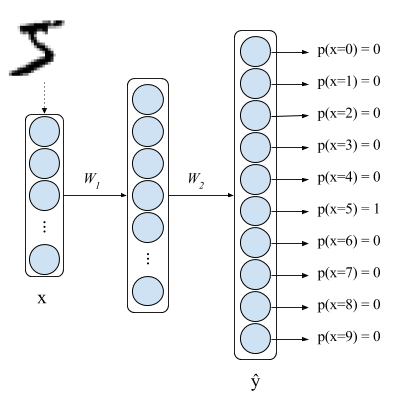
\includegraphics[scale=0.4,natwidth=400,natheight=406]{figures/supervisedLearning.png}
			\caption{Exemple avec un r\'eseau de neurones. L\textquotesingle entr\'ee $x$ correspond \`a l\textquotesingle image du nombre, et $\^y$ est la sortie souhait\'ee. Ici, le nombre est $5$, donc on souhaite que la sortie nous donne une probabilit\'e de $1$ pour $5$.}
				\label{fig:supervisedLearning}
		\end{figure}

	\subsection{S\'eries temporelle}
		Une s\'erie temporelle est un s\'erie qui \'evolue dans le temps. Ces s\'eries sont utilis\'ees dans de nombreux domaines, tels que la m\'edecine, la biologie, les mouvements \cite{ratanamahatana2004everything}, ... Les images peuvent aussi \^etre transform\'ees en s\'erie \cite{ratanamahatana2004everything}. Les s\'eries temporelles qui seront utilis\'ees lors ce stage seront tir\'ees des archives d\textquotesingle UCR \cite{UCRArchive}. 	

	\subsection{Ce qui ce fait actuellement}
	\label{seq:unknow}
		\subsubsection{Techniques bas\'ees sur la distance}
			Les techniques DTW ou ED sont des m\'ethodes permettant de comparer point-\`a-point diff\'erentes s\'eries temporelles (figure~\ref{fig:distance}). Ces deux techniques pr\'esentent chaucun leurs avantages et leurs inconvenients. Si l\textquotesingle ED est rapide \`a calculer, il n\textquotesingle est pas tr\`es efficace lorsque deux s\'eries sont dephas\'ees. Et si le DTW est efficace, il est plus complexe \`a mettre en place et demande plus ressources. Cependant, Ratanamahatana et Keogh \cite{ratanamahatana2005three} informe que le nombre de ressources mis en place pour faire fonctionner le DTW peuvent \^etre r\'eduites. 
			%La figure~\ref{fig:distance} illustre bien les diff\'erences entre ces deux m\'ethodes.

			\begin{figure}[!ht]
				\begin{subfigure}{0.45\textwidth}
					\centering	
					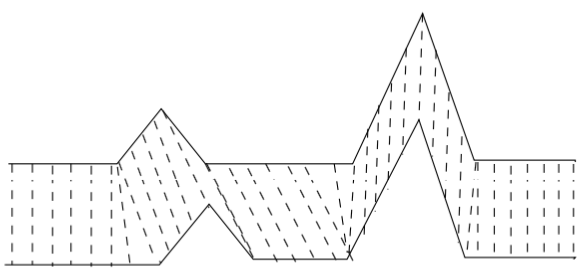
\includegraphics[scale= 0.6,natwidth=288,natheight=133]{figures/dtw.png}
					\caption{D\'eformation temporelle dynamique}
					\label{fig:dtw}
				\end{subfigure}
				\hspace*{\fill}
				\begin{subfigure}{0.45\textwidth}	
					\centering
					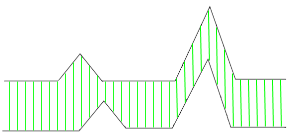
\includegraphics[scale= 0.6,natwidth=288,natheight=133]{figures/ed.png}
					\caption{Distance euclidienne}
					\label{fig:ed}
				\end{subfigure}
				\caption{Comparaison entre le DTW (\ref{fig:dtw}) et ED (\ref{fig:ed}).}
				\label{fig:distance}
			\end{figure}



		\subsubsection{Sac \`a mots}
		\label{seq:bagOfWords}
			Les sacs \`a mots (BoW en anglais pour \textit{Bag-of-Words}) sont un mod\`ele de description de document avec des descripteurs (qui sont consid\'er\'es comme des mots). Il fonctionne en attribuant des mots aux documents, chaque mot ayant une probabilit\'e par document (figure~\ref{fig:BoW}). L\textquotesingle article de Bailly et coll. \cite{bailly2015bag} traite justement le sujet de la classification des s\'eries temporelles avec les \textit{bag-of-words}. En utilisant les maximums et minimums locaux, ils obtiennent des mots qui seront ensuite utilis\'es dans la description des s\'eries temporelles.

			\begin{figure}[!ht]
				\centering
				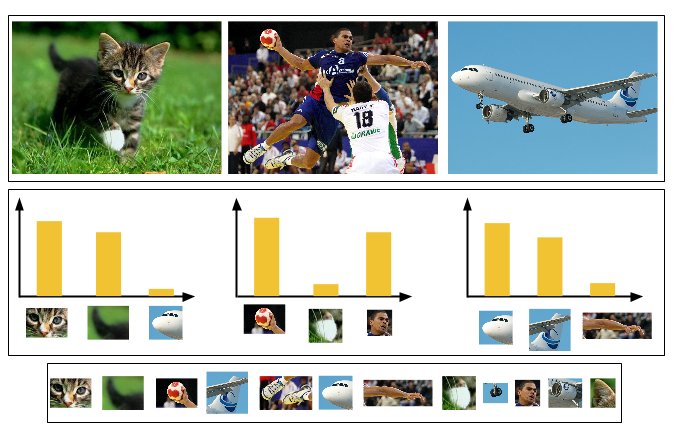
\includegraphics[scale=0.5,natwidth=680,natheight=440]{figures/bagOfWords.png}
				\caption{Le bag-of-words est en bas de la figure, il est compos\'e de diff\'erents mots, ici des images, qui sont reconnus sur les documents (en haut), qui sont ici des images. Par exemple, pour la premi\`ere image, on a une forte correspondance avec le premier et deuxi\`eme mot, alors que l\textquotesingle elle est faible correspondance avec la derni\`ere image.}
				\label{fig:BoW}
			\end{figure}

			En utilisant l\textquotesingle algorithme de SIFT (\textit{Scale-Invariant Feature Transform}) sur les donn\'ees d\textquotesingle UCR (\cite{UCRArchive}), les taux d\textquotesingle erreurs obtenus dans \cite{bailly2015bag} sont parfois meilleurs qu'en utilisant la m\'ethode des k plus proches voisins seuls coupl\'e avec le DTW.
			Pour cr\'eer des mots, plusieurs m\'ethode.

	\subsection{R\'eseau de neurones}
	\label{seq:neuralNetwork}
		Les r\'eseaux de neurones sont un syst\`eme inspir\'e du mod\`ele biologique du cerveau. Un r\'eseau de neurones est compos\'e de plusieurs neurones (figure~\ref{fig:neuralNetwork}) qui ont chacun une fonction d\textquotesingle activation (figure~\ref{fig:neural}) et qui sont reli\'es \`a d\textquotesingle autres neurones par des poids.

		\subsubsection{Un r\'eseau de neurones en g\'en\'eral}
		\label{seq:simpleNeuralNetwork}
			\begin{itshape}Les neurones\end{itshape}

			\begin{equation}
				f(x) = \frac{1}{1 + \exp{-x}}
				\label{eq:sigmoid}
				\caption{Exemple d\textquotesingle activation : Une sigmo\¨ide}
			\end{equation}

			Un neurone est une unit\'e qui contient une fonction d\textquotesingle activation qui d\'efinit son comportement. La figure~\ref{fig:neural} repr\'esente un neurone qui a 4 entr\'ees et une sortie. On note \texbf{$X$} le vecteur d\textquotesingle entr\'ee, \textbf{$W$} le vecteur des poids, $b$ le biais, $f(.)$ la fonction d\textquotesingle activation (\'equation~\ref{eq:sigmoid}), et $h(X)$ la sortie du neurone. Notons aussi $z$ la somme des poids et $n$ le nombre d\textquotesingle entr\'ees d\textquotesingle un neurone (sans compter le biais). On a donc les \'equations suivantes :
			
			\begin{equation}
				z = \sum_{k=0}^n w_k x_k + b
				\label{eq:z}
			\end{equation}

			\begin{equation}
				h_{W,b}(X) = f(z)
				\label{eq:h}
			\end{equation}

			\begin{figure}[!ht]
				\centering
				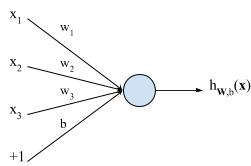
\includegraphics[scale=0.5,natwidth=251,natheight=166]{figures/neural.png}
				\caption{Comme on peut le voir, le neurone ci-dessus re\c coit 4 valeurs, dont le biais. Dans un r\'eseau de neurones, les entr\'ees $x$ sont les sorties d\textquotesingle autres neurones.}
				\label{fig:neural}
			\end{figure}

			Un neurone seul ne peut pas effectuer de t\^ache, c\textquotesingle est pourquoi ils sont utilis\'es \`a plusieurs pour effectuer diverses t\^aches comme de l\textquotesingle analyse de donn\'ee ou de la classification.	

			\medbreak
			\begin{itshape}L\textquotesingle architecture\end{itshape}

			L\textquotesingle efficacit\'e d\textquotesingle un r\'eseau de neurones d\'epend de son architecture.
			Il existe diff\'erentes architectures pour un r\'eseau de neurones (figure~\ref{fig:neuralNetwork}), la plus connue et la plus r\'epandue \'etant le r\'eseau de neurones non boucl\'es (ou feedfoward neural network en anglais) (figure~\ref{fig:nnl}). Selon le nombre de couche cach\'ee et le nombre de neurones par couche, le r\'eseau peut \^etre plus ou moins performant (\cite{chatfield2014return}, \cite{srivastava2014dropout}). 

			\begin{figure}[!ht]
				\centering
				\begin{subfigure}{0.45\textwidth}
					\centering	
					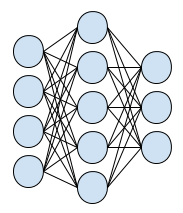
\includegraphics[scale=0.7,natwidth=183,natheight=213]{figures/neuralNetworkLayers.png}
					\caption{R\'eseau de neurones \`a couche}
					\label{fig:nnl}
				\end{subfigure}
				\hspace*{\fill}
				\begin{subfigure}{0.45\textwidth}	
					\centering
					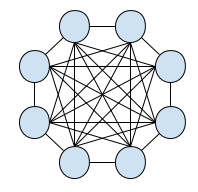
\includegraphics[scale=0.7,natwidth=198,natheight=192]{figures/neuralNetworkCompleteConnexion.png}
					\caption{R\'eseau de neurones \`a connexion compl\`ete}
					\label{fig:nnc}
				\end{subfigure}
				\caption{Il existe diff\'erents types de r\'eseaux de neurones. Par exemple, la figure 1.a est un r\'eseau avec une architecture \`a couche, alors que le r\'eseau de la figure 2.b \`a une architecture \`a connexion compl\`ete. Dans le domaine de la classification, l\textquotesingle architecture \`a couche est souvent utilis\'ee.}
				\label{fig:neuralNetwork}
			\end{figure}
			
			Pour faire fonctionner un r\'eseau de neurones non boucl\'es, on lui transmet une entr\'ee qui est de la m\^eme taille que la couche d\textquotesingle entr\'ee (par exemple, si l\textquotesingle entr\'ee est une image, sa taille peut correspondre au nombre de pixel). Ces valeurs sont ensuite transmises aux neurones de la couche suivante de mani\`ere r\'epet\'ee jusqu\textquotesingle \`a couche de sortie.

			En appliquant les formules \ref{eq:z} et \ref{eq:h}, et en notant $L$ le nombre de couche dans le r\'eseau, $a$ l\textquotesingle activation d\textquotesingle un neurone (qui correspond \`a la sortie du neurone), $n^{(l)}$ le nombre de neurones de la couche $l$, $w_{ij}^{(l)}$ le poids allant du neurone $j$ de la couche $l-1$ au neurone $i$ de la couche $l$, $x$ le vecteur d\textquotesingle entr\'ee du r\'eseau, on obtient les \'equations suivantes :

			\begin{equation}
				a_i^{(0)} = x_i
				\label{eq:input}
			\end{equation}

			\begin{equation}
				z_i^{(l)} = \sum_{k=0}^{n^{(l-1)}} w_{ik}^{(l)} a_k^{(l-1)} \enskip \forall 1 < l \leq L
				\label{eq:zGlobal}
			\end{equation}

			\begin{equation}
				a_i^{(l)} = f(z_i^{(l)}) \enskip \forall 1 < l \leq L
				\label{eq:activation}
			\end{equation}

			\medbreak
			\begin{itshape}L\textquotesingle apprentissage d\textquotesingle un r\'eseau de neurones\end{itshape}

			L\textquotesingle objectif de l\textquotesingle apprentissage est de trouver les poids qui lient les neurones. Le m\'ethode la plus souvent utilis\'ee est la backpropagation qui consiste \`a diminuer l\textquotesingle erreur de la sortie, l\textquotesingle erreur \'etant la diff\'erence entre la valeur obtenue et la valeur souhait\'ee dans le cas d\textquotesingle un apprentissage supervis\'e. Cette diff\'erence est aussi appel\'e la fonction de co\^ut et est not\'e $J(W,b;x,y)$ avec $W$ la matrice des poids, $b$ le vecteur des biais, $x$ le vecteur d\textquotesingle entr\'ee, et $y$ le vecteur de sortie esp\'er\'e. Le but est donc bien de diminuer au maximum cette fonction de co\^ut. Dans le tutoriel de Ng et coll. (\cite{ng2012ufldl}), cette fonction de co\^ut est d\'ecrite par l\textquotesingle equation suivante :

			\begin{equation}
				J(W,b;x,y) = \frac{1}{2} {\left\Vert h_{W,b}(x) - y \right\Vert}^2
				\label{eq:costFunction}
			\end{equation}

			Une fois cette fonction trouv\'ee, on applique une descente de gradient sur les param\`etres $W$ et $b$. On a donc :

			\begin{equation}
				W_{ij}^{(l)} = W_{ij}^{(l)} - \alpha \frac{\partial}{\partial W_{ij}^{(l)}} J(W,b)
				\label{eq:gradientDescentWeight}
			\end{equation}
 
			\begin{equation}
				b_{i}^{(l)} = b_{i}^{(l)} - \alpha \frac{\partial}{\partial b_{i}^{(l)}} J(W,b)
				\label{eq:gradientDescentBiaises}
			\end{equation}

			$\alpha$ correspond au taux d\textquotesingle apprentissage et doit \^etre soigneusement choisi. Si $\alpha$ est trop grand, on risque de louper les bonnes valeurs. Si $\alpha$ est trop petit, l\textquotesingle apprentissage sera plus long, mais on risque surtout de rester bloquer dans un extremum local. Pour r\'esumer les formules (\ref{eq:costFunction}), (\ref{eq:gradientDescentWeight}) et (\ref{eq:gradientDescentBiaises}), on part de la sortie du r\'eseau de neurones pour revenir jusqu\textquotesingle \`a l\textquotesingle entr\'ee tout en modifiant sur le chemin les poids qui relient les neurones entre chaque couche. On relance ensuite le r\'eseau de neurones avec la m\^eme donn\'ee.
			On recommence ce processus selon diverses conditions, comme un nombre fix\'e \`a l\textquotesingle avance, un taux d\textquotesingle erreur atteint, ...
			On relance tout ce processus autant de fois que l\textquotesingle on a de donn\'ees d\textquotesingle entra\^inement.

			Dans le cas d\textquotesingle un apprentissage non supervis\'e, une des m\'ethodes utilis\'ees est d\textquotesingle entra\^iner, de la m\^eme mani\`ere qu'un r\'eseau classique, un autoecoder. Un autoencoder est un r\'eseau de neurones o\`u la sortie est approximativement \'egale \`a l\textquotesingle entr\'ee (figure~\ref{fig:autoencoder}). On essaye donc de trouver la fonction $h_{W,b}(x) \approx x$. Le r\'eseau autoencoder apprend donc \`a trouver les axes principaux de la donn\'ee d\textquotesingle entr\'ee \cite{hinton2006reducing} (de la m\^eme mani\`ere que l\textquotesingle ACP).

			\begin{figure}[!ht]
				\centering
				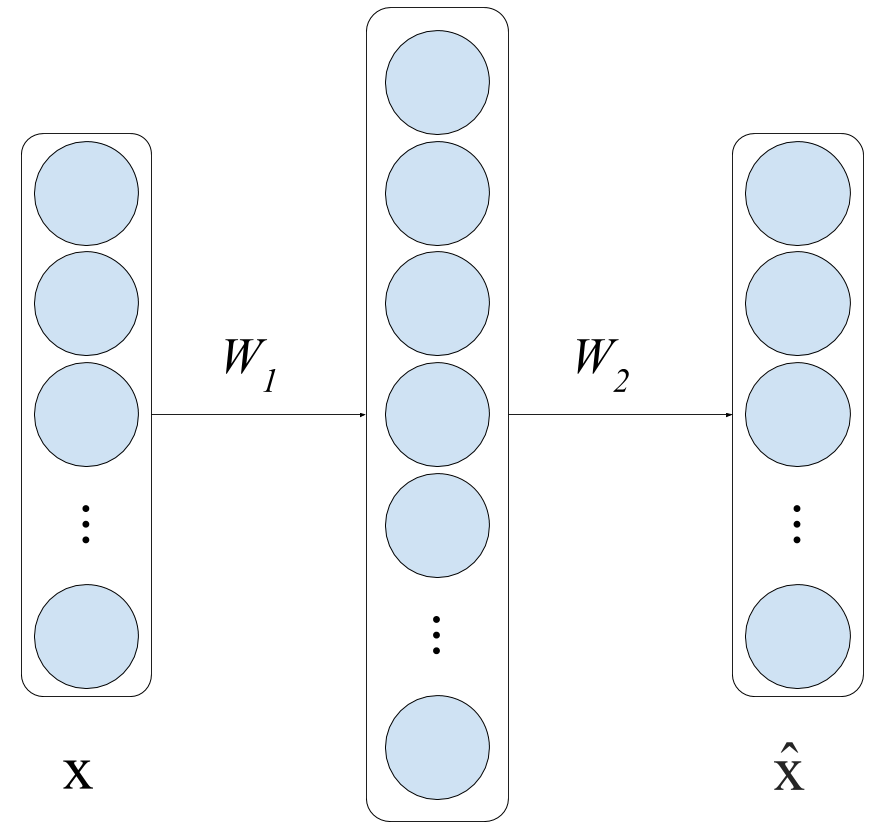
\includegraphics[scale=0.15,natwidth=893,natheight=837]{figures/autoencoder.png}
				\caption{$x$ est \textquotesingle entr\'ee, et $\^x$ est une approximation de l\textquotesingle entr\'ee appliqu\'ee sur la sortie.}
				\label{fig:autoencoder}
			\end{figure}

			



			\medbreak

		\subsubsection{R\'eseau de neurones profond}
		\label{seq:DeepNetwork}
			Un r\'eseau de neurones profond est un r\'eseau qui contient plusieurs couches cach\'ees. Ce type de r\'eseau a l\textquotesingle avantage de pouvoir apprendre un plus grand nombre de fonctions avec un nombre de neurones bien inf\'erieurs dans les couches cach\'ees \`a celui d\textquotesingle un r\'eseau classique. En effet, \`a la place d\textquotesingle avoir un nombre exponentiel de neurones cach\'es (par rapport aux neurones d\textquotesingle entr\'ees), nous avons un nombre polynomial.
			
			Cependant, les r\'eseaux de neurones profonds sont plus difficiles \`a entra\^iner qu\textquotesingle un r\'eseau classique, car ils n\'ecessitent beaucoup de donn\'ees label\'ees pour l\textquotesingle entra\^inement du r\'eseau \cite{krizhevsky2012imagenet}\cite{howard2013some}. L\textquotesingle entra\^inement d\textquotesingle un r\'eseau avec peu de donn\'ees m\`enerait un sur-apprentissage (figure~\ref{fig:overfitting}). 
			En plus du manque de donn\'ees, l\textquotesingle entra\^inement par backpropagation vu \`a la section \ref{seq:simpleNeuralNetwork} est peu efficace s\textquotesingle il est utilis\'e tel quel, et m\`ene souvent au sur-apprentissage (due aux extremums locaux). Il faut donc les entra\^iner diff\'erement.

			Il ne faut donc pas initialiser les poids al\'eatoirement, mais les initialiser \`a une valeur plus juste par un pr\'e-entra\^inement. Pour cela, on va utiliser l\textquotesingle algorithme du \textit{greedy layerwise training} sur un r\'eseau de neurones \textit{stacked autoencoder}. 
			L\textquotesingle algorithme \textit{greedy layer-wise} consiste d\textquotesingle abord entra\^iner un r\'eseau avec une couche cach\'ee par \textit{backpropagation}, de garder les param\`etres obtenus, puis de rajouter une seconde couche cach\'ee, et ainsi de suite.
			Selon le type d\textquotesingle apprentissage (supervis\'e ou non), la sortie souhait\'ee \`a chacune de ces \'etapes est la couche cach\'ee pr\'ecedente ({figure~\ref{fig:pretrainingDeepNet}). Un fois ce pr\'e-entra\^inement termin\'e, on peut commencer l\textquotesingle entra\^inement du r\'eseau par \textit{backpropagation}.

			\begin{figure}[!ht]
				\centering
				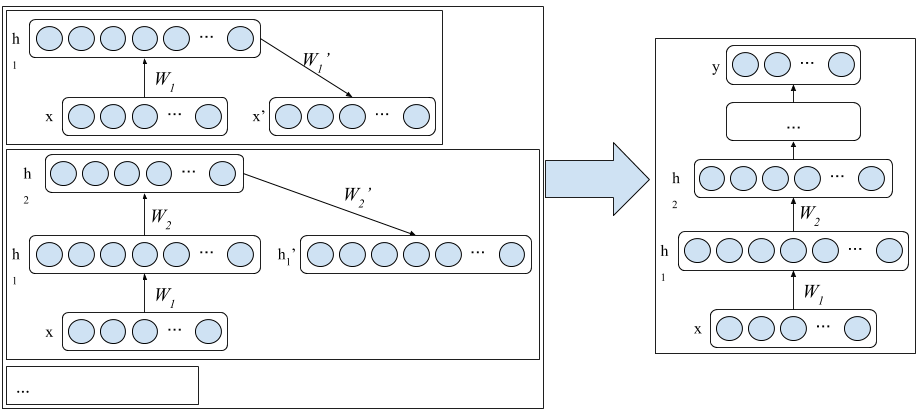
\includegraphics[scale=0.4,natwidth=919,natheight=412]{figures/trainDeepNetByGreedyLayerWiseUnsupervised.png}
				\caption{Entra\^inement d\textquotesingle un r\'eseau de neurones profond pour un apprentissage non supervis\'e.}
				\label{fig:pretrainingDeepNet}
			\end{figure}

		\subsubsection{R\'eseau de neurones convolutionnels}
		\label{seq:CNN}
			Les CNN (Convolutional Neural Network, ou r\'eseaux de neurones convolutionnels) sont une structure particuli\`ere des r\'eseaux de neurones profonds car les neurones d\textquotesingle une couche \`a une autre ne sont pas tous reli\'es entre eux. En effet, ses connexions entre neurones se font localement, ce qui fait des entr\'ees d\textquotesingle une couche cach\'ee un sous-ensemble de motif de la couche pr\'ec\'edente (figure~\ref{fig:cnn}.

			\begin{figure}[!ht]
				\centering
				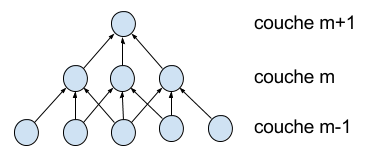
\includegraphics[scale=0.5,natwidth=375,natheight=152]{figures/architectureCNN.png}
				\caption{Ici, imaginons que la couche m-1 est une r\'etine o\`u chaque neurone correspond \`a un pixel d\textquotesingle une image. Dans la couche m, on s\textquotesingle aper\c coit que chaque neurone a 3 entr\'ees qui correspondent chacune \`a un pixel. Chaque neurone de la couche m est donc un sous-ensemble de l\textquotesingle image de 3 pixels. De la m\^eme fa\c con, chaque neurone de la couche m+1 est donc un sous-ensemble de l\textquotesingle image de 5 pixels.}
				\label{fig:cnn}
			\end{figure}

			Dans la figure~\ref{fig:cnn}, les neurones de la couche m-1 sont les filtres de cette couche. De la m\^eme fa\c con, les neurones de la couche m-2 sont aussi des filtres de cette couche. Un CNN peut avoir plusieurs couches de filtres, le nombre de filtres d\'ecroissant d\textquotesingle une couche \`a une autre.
			Appliqu\'es \`a une image, les filtres de la premi\`ere couche cach\'ee peuvent \^etre associ\'es \`a un ensemble de pixels (figure~\ref{fig:cnnChat}), et ensuite de suite avec les autres couches.

			\begin{figure}[!ht]
				\centering
				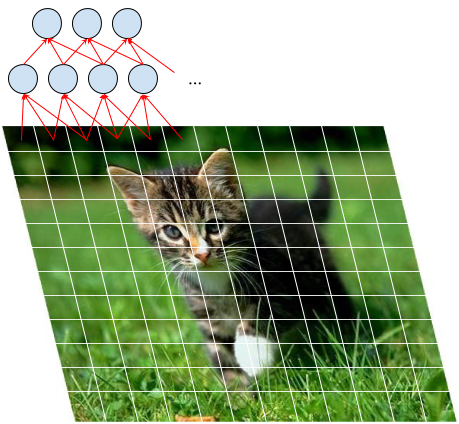
\includegraphics[natwidth=474,natheight=504,scale=0.4]{figures/cnnOnImage.png}
				\caption{L\textquotesingle image d\textquotesingle entr\'ee contient ici 144 composantes, donc la couche d\textquotesingle entr\'ee contiendra 144 neurones. On peut voir que la premi\`ere couche cach\'ee est bien un ensemble de pixels.}
				\label{fig:cnnChat}
			\end{figure}

			Pour les s\'eries temporelles, les CNN peuvent aussi s\textquotesingle appliquer. Par exemple, l\textquotesingle article de Zheng et coll. (\cite{zheng2014time}) utilise les CNN pour faire de la classification de s\'eries temporelles multivari\'ees, c\textquotesingle est-\`a-dire des s\'eries temporelles qui sont sur plusieurs dimensions.

			\medbreak
			\begin{itshape}Pooling\end{itshape}

			On peut imaginer que la figure~\ref{fig:cnnChat} nous montre une image avec 144 pixels, que chaque filtre prend un zone de 1x3 pixels (comme sur la figure), et que nous voulons apprenndre 400 fonctions pour chaque zone de pixels, on se retrouve avec (12 - 3 + 1)(13 - 1 + 1) x 400 = 48 000 fonctions \`a apprendre. Apprendre 48 000 fonctions n\textquotesingle est pas difficile pour un ordinateur. Cependant, si l\textquotesingle image fait 100x100 pixels, qu\textquotesingle on \'elargit les zones de filtre \`a 5x5 pixels par exemple, on obtient (100 - 5 + 1)(100 - 5 + 1) x 400 = 3 686 400 fonctions \`a apprendre. Apprendre une telle quantit\'e de fonction est tr\`es lent et augmente surtout le risque de sur-apprentissage.


			Pour \'eviter cela, on  peut utiliser le \textit{pooling}. Tr\`es utile pour utiliser les CNN, le \textit{pooling} va r\'eduire significativement le nombre de filtres pr\'esent dans un r\'eseau de neurones convolutionnel. Par exemple, pour image, on va s\'electionner des zones de pixels al\'eatoirement qui passeront \`a un autoencoder. Il est important de pr\'eciser qu\textquotesingle il ne doit y avoir aucun recouvrement. Une fois les filtres appris, on pourra utiliser les CNN avec les images enti\`eres. Ensuite, selon le \textit{pooling} choisi, par exemple le \textit{max-pooling}, on  prendra le maximum de toutes les r\'eponses de filtres. On r\'eduit donc ainsi le nombre de fonctions \`a apprendre.
			Par exemple, si on garde les 400 fonctions \`a apprendre par filtre, la figure~\ref{fig:maxpooling} donnera 4800 fonctions \`a apprendre, au lieu de 48000 pour la figure~\ref{fig:cnnChat}.

			\begin{figure}[!ht]
				\centering
				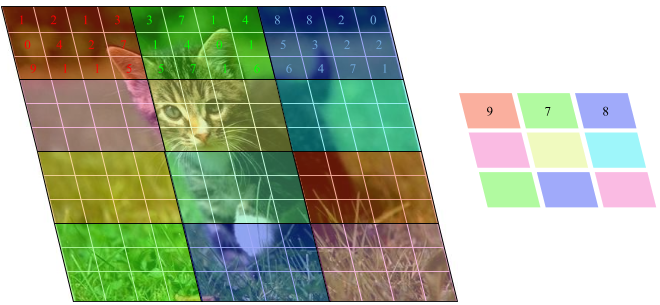
\includegraphics[natwidth=650,natheight=305,scale=0.4]{figures/maxPooling.png}
				\caption{Exemple de \textit{max-pooling} avec des zones de 3x4 pixels.}
				\label{fig:maxpooling}
			\end{figure}

	\subsection{Le manque de donn\'ee}
	\label{seq:noData}

		\subsubsection{Sur-apprentissage et sous-apprentissage}
			\begin{itshape}Sur-apprentissage\end{itshape}

			L\textquotesingle apprentissage conna\^it deux probl\`emes principaux, le sur-apprentissage (overfitting en anglais) et le sous-apprentissage (underfitting en anglais).
			Le sur-apprentissage appara\^it lorsque le r\'eseau de neurones s\textquotesingle est trop sp\'ecialis\'e. Cela arrive lorsque l\textquotesingle on entra\^ine le r\'eseau trop de fois sur le m\^eme jeu de donn\'ees. Par exemple, la figure~\ref{fig:overfitting} montre un exemple de sur-apprentissage, la courbe rouge \'etant bien capable de retrouver les donn\'ees d\textquotesingle entra\^inement, mais serait incapable de retrouver une donn\'ee se situant sur la courbe verte.

			\begin{itshape}Sous-apprentissage\end{itshape}
			Le sous-apprentissage est lui un probl\`eme de manque d\textquotesingle entra\^inement. Comme on peut le voir sur la figure~\ref{fig:underfitting}, la courbe rouge ne s\textquotesingle est pas assez sp\'ecialis\'ee contrairement au cas du sur-apprentissage.

			C\textquotesingle est pourquoi la taille de la base de donn\'ees utilis\'ee influence beaucoup les r\'esultats.


			\begin{figure}[!ht]
				\centering
				\begin{subfigure}{0.45\textwidth}
					\centering
					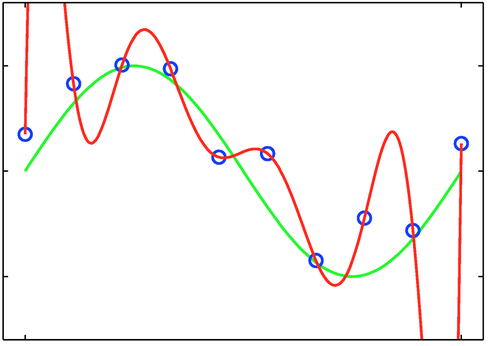
\includegraphics[natwidth=489,natheight=346,width=200,height=140]{figures/overfitting.png}
					\caption{Sur-apprentissage}
					\label{fig:overfitting}
				\end{subfigure}
				\hspace*{\fill}
				\begin{subfigure}{0.45\textwidth}	
					\centering
					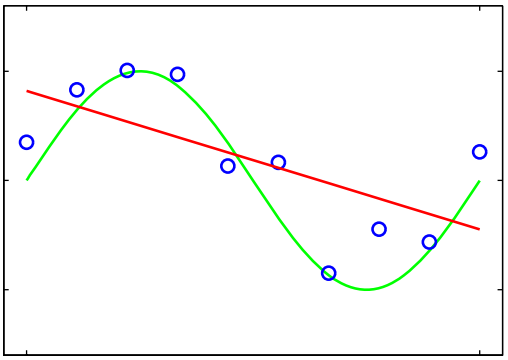
\includegraphics[natwidth=508,natheight=360,width=200,height=140]{figures/underfitting.png}
					\caption{Sous-apprentissage}
					\label{fig:underfitting}
				\end{subfigure}
				\caption{Les points bleus sont les donn\'ees \`a apprendre, la courbe verte est la fonction que l\textquotesingle on aimerait avoir, et la courbe rouge est la fonction que l\textquotesingle on a obtenue.}
			\end{figure}

		\subsubsection{L\textquotesingle augmentation de donn\'ees}
		\label{seq:dataAugmentation}
			\medbreak

			\begin{itshape}{Pourquoi chercher \`a augmenter la base de donn\'es ?}\end{itshape}

			On a besoin de pallier le manque de donn\'ees car les architectures de r\'eseau de neurones profonds, comme les CNN, ont besoin de beaucoup de donn\'ees pour pouvoir \^etre entra\^in\'es efficacement. Les structures telles que MC-DCNN de Zheng et coll. (\cite{zheng2014time}) peuvent \^etre utilis\'ees.
			De plus il y a peu, compar\'e aux images, de donn\'ees label\'ees sur les s\'eries temporelles. On aura donc besoin d\textquotesingle augmenter ces donn\'ees de diff\'erentes fa\c cons.
			Par analogie aux images, on regardera comment transformer une s\'erie temporelle. Dans les donn\'ees pour les images, on applique certaines transformations (\cite{krizhevsky2012imagenet}\cite{howard2013some}), tel que la translation, l\textquotesingle inversion, le changement de couleur, de contraste, de luminosit\'e, ... (figure~\ref{fig:dataAugmentationChat}). Ces transformations ne sont pas forc\'ement applicables aux s\'eries temporelles et on regardera donc comment faire.

			\medbreak

			\begin{itshape}{Comment y parvenir ?}\end{itshape}
			
			Pour les images, plusieurs techniques existent. Par exemple, Chatfield et coll. (\cite{chatfield2014return}) explique que pour r\'ealiser une augmentation de donn\'ees, ils perturbent une image avec des transformations qui n\textquotesingle invalident pas cette image, c\textquotesingle est-\`a-dire que si l\textquotesingle image d\textquotesingle origine montrait un chat, l\textquotesingle image transform\'ee doit toujours montrer un chat. Krizhevsky et coll. (\cite{krizhevsky2012imagenet}) explique que pour augmenter ses donn\'ees, il s\'epare tout d\textquotesingle abord ses donn\'ees en deux parties, l\textquotesingle une pour l\textquotesingle apprentissage, et l\textquotesingle autre pour les tests. Dans les donn\'ees pour l\textquotesingle apprentissage, ils r\'ealisent des sous-images en extractant des zones de 224x224 pixels de l\textquotesingle image d\textquotesingle origine et de sa r\'eflection horizontale, qui a une taille de 256x256. On obtient donc une multiplication de 2048 de la base de donn\'ees d\textquotesingle origine. Les donn\'ees de test prendront 5 sous-images et leur r\'eflection (donc 10 images) selon leurs pr\'edictions. Toujours dans l\textquotesingle id\'ee d\textquotesingle augmenter leurs donn\'ees d\textquotesingle apprentissage, ils effectuent une ACP pour pouvoir, non pas r\'eduire les dimensions, ajouter du bruit contr\^ol\'e sur les composants principaux. Krizhevsky et coll. ([5]) arrivent donc \`a baisser le taux d\textquotesingle erreur de plus de 1\% ainsi. Dans le papier [6], Howard utilise le m\^eme proc\'ed\'e mais rajoute d\textquotesingle encore d\textquotesingle autres \'etapes. 

			\begin{figure}[!ht]
				\centering
				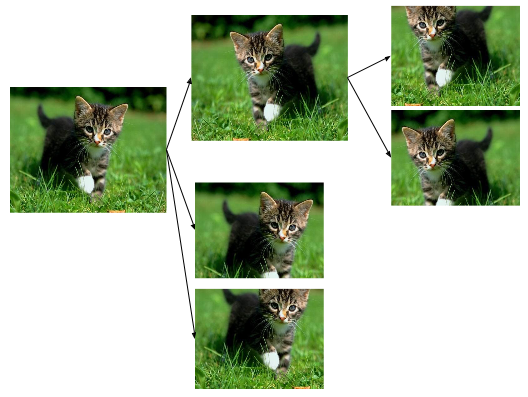
\includegraphics[scale=0.5,natwidth=528,natheight=397]{figures/dataAugmentationImage.png}
				\caption{Exemple d\textquotesingle augmentation de donn\'ees pour une image. Ici, on a obtenu six images \`a partir d\textquotesingle une seule. On a d\textquotesingle abord appliqu\'e une inversion d\textquotesingle image et puis on a rogn\'e les images obtenues de deux mani\`eres diff\'erentes. En r\'ealit\'e, beaucoup plus de transformations sont appliqu\'ees, permettant de multiplier la base de donn\'ees des images de beaucoup (1024 dans~\cite{howard2013some}).}
				\label{fig:dataAugmentationChat}
			\end{figure}

			Beaucoup de m\'ethode de data-augmentation le sont pour les images, la question \'etant de savoir si parmi ces m\'ethodes, on peut en r\'eutiliser ou non. Par exemple, on ne peut pas r\'ealiser une r\'eflection sur une s\'erie temporelle. Cependant, l\textquotesingle approche de Krizhevsky dans \cite{krizhevsky2012imagenet} pour les donn\'ees d\textquotesingle entra\^inement avec une ACP pourrait \^etre r\'ealisable sur des s\'eries temporelles. On pourrait peut-\^etre aussi rajouter du bruit contr\^ol\'e selon diff\'erents param\`etres comme dans \cite{krizhevsky2012imagenet} ou \cite{howard2013some}.

		\subsubsection{Dropout}
		\label{seq:dropout}
			Le dropout (vient de la contraction de deux mots anglais \textit{dropping out}) est une m\'ethode d\textquotesingle apprentissage qui permet d\textquotesingle obtenir de bons r\'esultats avec un nombre de donn\'ees r\'eduites. L\textquotesingle article de Srivastava et coll. (\cite{srivastava2014dropout}) introduite cette notion. Le principe est de d\'esactiver certains neurones par couche al\'eatoirement (figure~\ref{fig:dropout}).

			\begin{figure}[!ht]
				\centering
				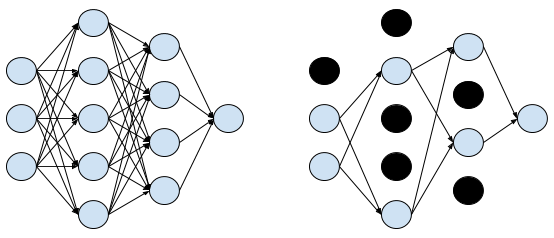
\includegraphics[scale=0.6,natwidth=554,natheight=238]{figures/dropout.png}
				\caption{Le r\'eseau de neurones \`a droite est celui de gauche apr\`es que l\textquotesingle on ait appliqu\'e le dropout. Comme on peut le voir, on r\'eduit de beaucoup le nombre de connexions entre les neurones.}
				\label{fig:dropout}
			\end{figure}

			On applique en fait une probabilit\'e \`a chaque couche. Par exemple, une probabilit\'e de 0.5 sur la couche $l$ d\textquotesingle un r\'eseau de neurones signifie que les neurones de cette couche ont chacun une probabilit\'e de 0.5 d\textquotesingle \^etre activ\'e. On note cette probabilit\'e $p$ et on a donc la formule~(\ref{eq:zGlobal}) qui devient :

			\begin{equation}
				r_j^{(l)} ~~ Bernouilli(p)
				\label{eq:bernouilli}
			\end{equation}

			\begin{equation}
				\~a^{(l)} = r^{(l)} * a^{(l)}
				\label{eq:activationDropout}
			\end{equation}

			\begin{equation}
				z_i^{(l)} = \sum_{k=0}^{n^{(l-1)}} w_{ik}^{(l)} \~a_k^{(l-1)} \enskip \forall 1 < l \leq L
				\label{eq:zDropout}
			\end{equation}

			On comprend donc que la probabilit\'e $p$ est une valeur influence l\textquotesingle efficacit\'e du dropout. En effet, si $p$ est trop grand (proche de 1), on se rapproche trop d\textquotesingle un apprentissage classique, et ne pr\'esente donc peu d\textquotesingle inter\^et. Au contraire, si $p$ trop petit, le r\'eseau aura beaucoup de difficult\'e \`a apprendre car il y a trop peu de neurone pr\'esent. Srivastava et coll. (\cite{srivastava2014dropout}) nous informe que choisir $p = 0.5$ donne en g\'en\'eral de bons r\'esultats.

			On peut entra\^iner un r\'eseau de neurones en combinant le dropout et la \textit{backpropagation}, mais cette \textit{backpropagation} n\textquotesingle est pas appliqu\'ee au r\'eseau tout entier, mais \`a un r\'eseau ``aminci'' par le dropout. Les poids sont alors partag\'es entre chaque r\'eseau de neurones aminci. \'Etant donn\'e que l\textquotesingle on doit g\'en\'erer plusieurs r\'eseaux amincis, il n\textquotesingle est pas \'etonnant que cette entra\^inement prend plus de temps qu\textquotesingle un r\'eseau de neurones classique. En effet, entra\^iner un r\'eseau de neurones avec le dropout prend 2 \`a 3 fois plus de temps \cite{srivastava2014dropout}.
			Lors du test, il faut alors multiplier tous les poids par $p$ sur le r\'eseau entier.

			Le taux d\textquotesingle erreur observ\'e est significativement plus petit en utilisant le dropout que sans \cite{srivastava2014dropout}. De plus, le dropout permet de pr\'evenir l\textquotesingle apparition de sur-apprentissage.


\bigbreak
\bigbreak
\section{Conclusion}
\label{seq:conclusion}
Pour conclure , il existe de nombreuses mani\`eres d\textquotesingle augmenter le volume des donn\'ees. Cependant, ces m\'ethodes d\'ependent du type de donn\'ee. Avant de commencer \`a classifier des s\'eries temporelles, il va donc falloir trouver comment augmenter ce volume. Nous pourrions, par exemple, utiliser l\textquotesingle algorithme ACP ou s\textquotesingle inspirer des m\'ethodes utilis\'ees sur les images.
Pour la classification, les CNN semblent \^etre un bon choix \'etant donn\'e les bons r\'esultats obtenus par Zheng et coll. (\cite{zheng2014time}). Pour cela, nous allons utiliser le framework Caffe (voir \cite{jia2014caffe}). Une fois mis en place, nous pourrions alors observer les r\'esultats.



\nocite{*}
\bibliographystyle{plain}
\bibliography{biblio}



\end{document}
%%% Local Variables:
%%% mode: latex
%%% TeX-master: t
%%% End:
